\chapter{General}
\section{Scope}
Example of equation reference: Eq.\eqref{eq:test}.
\begin{equation}\label{eq:test}
    A=\dfrac{B^2}{\gamma_0}
\end{equation}

Example of citation within text: \textcite{Jensen1906}\par
Example of citation in parenthesis:
\parencite{Hasofer1974}

An example of a figure is Figure~\ref{fig:lifecycle}:
\begin{figure}[h!]
  \centering
    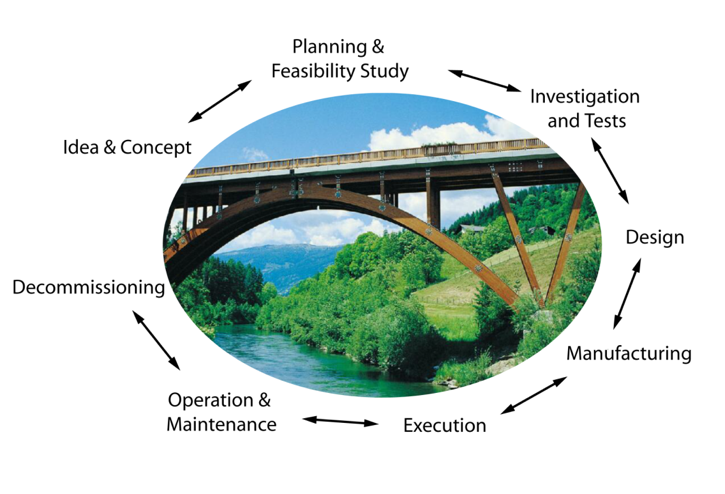
\includegraphics[width=0.7\textwidth]{./example_fig.png}
    \vspace*{-20pt}\caption{The life-cycle of engineering structures.}
    \label{fig:lifecycle}
\end{figure}

An example of a table is Table~\ref{tab:tab1}:
\begin{table}[h!]
  \caption{Parameter values.}
  \label{tab:label}
  \centering
    \begin{tabular}{|c|c|c|}
      \hline
      a & b & c \\
      \hline
      1.0 & 2.0 & 3.0 \\
      \hline
    \end{tabular}
    \label{tab:tab1}
\end{table}
